\documentclass[aspectratio=169]{beamer}
\usetheme{Hannover}
\usecolortheme{magpie}
\beamertemplatenavigationsymbolsempty
\usepackage{graphicx}
\graphicspath{{images}{scripts}}
\usepackage{tikz}
\usepackage{pgfplots}
\pgfplotsset{compat=1.18}
\title{{\it Distributional Emulation}}
\subtitle{Robust \& Rapid Emulation for Efficient Trial Design}
\author[]{Dr Jack Fraser-Govil \& Prof. Sam Watson}
\date{30/06/26}
% \logo{
\includegraphics[scale=0.3]{crest3}}
\makeatletter \addtobeamertemplate {sidebar left} {}{ 
\includegraphics [width=\beamer@sidebarwidth]{crest3}} \makeatother 

\renewcommand{\vec}[1]{\mathbf{\boldsymbol{#1}}}

\def\pitem{\pause\item}

\begin{document}
	\maketitle

	\section{Why Emulate?}
		\begin{frame}{Why do we want to Emulate?}

			\begin{itemize}
				\pitem Suppose we have some computational model of the effect of an intervention
				$$ \vec{y} = \hat{M}(\vec{\pi})$$
				\pitem Then suppose we wish to compute some complex quantity - such as the predictive power
				$$  p = \sum_\text{permutations} \sum_{\vec{\pi}} f(\vec{y}(\vec{\pi}))$$
			\end{itemize}

			\pause\begin{block}{The problem}
				\centering \large If $\hat{M}$ is slow (minutes-to-hours), it will take years-to-decades to compute $p$.
			\end{block}
		\end{frame}

		\begin{frame}{Why do we want to Emulate?}
			\begin{block}{What is an Emulator?}
				\centering \large An emulator is a function $\hat{E}_M$ which \textit{behaves} like $\hat{M}$, but which is vastly quicker to compute.
			\end{block}

		\end{frame}
	\section{Background Theory}
		\begin{frame}{Estimators, Regression}
			This is not a new idea!
			\vspace{1cm}

			\only<2>{ \centering 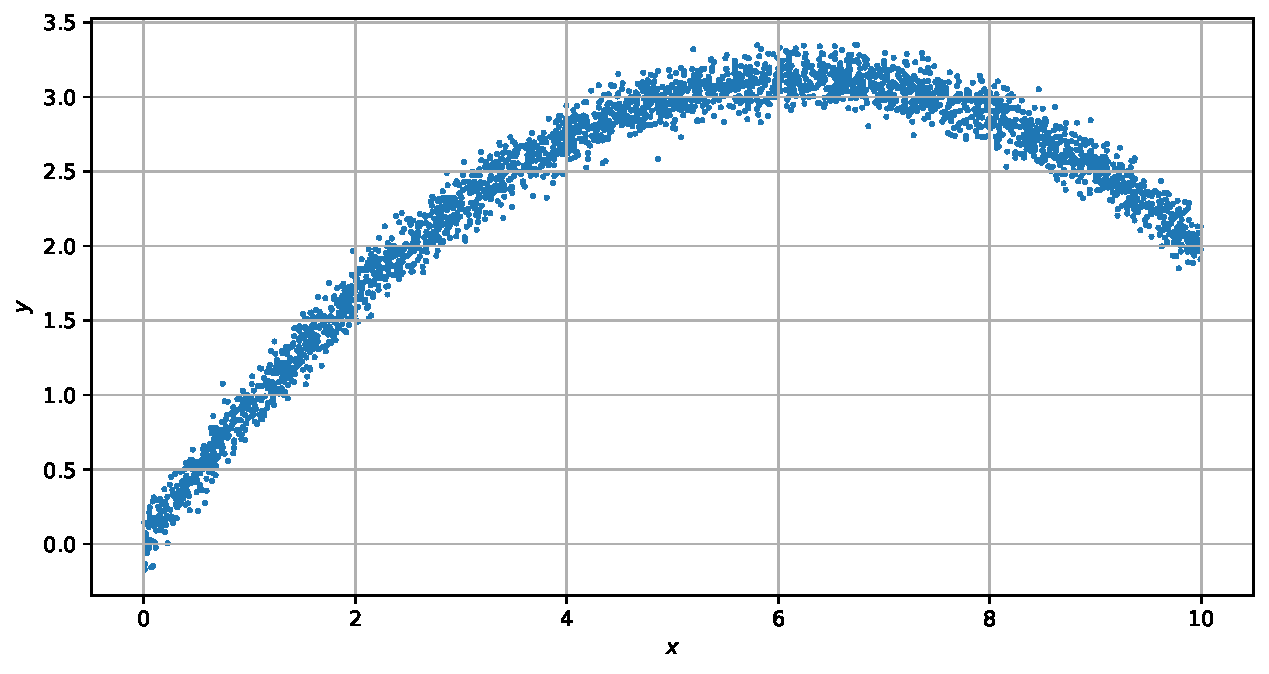
\includegraphics[width=\linewidth,height=0.6\paperheight,keepaspectratio=true]{data-only-f0.pdf}}
			\only<3>{ \centering 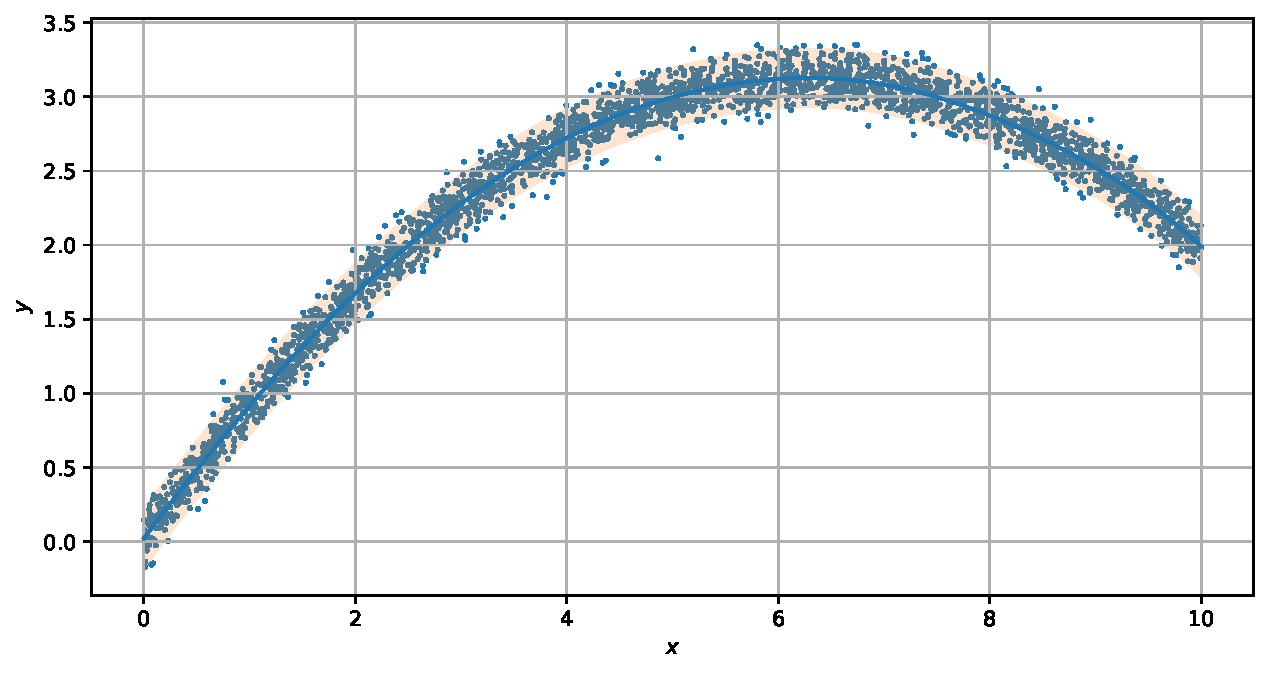
\includegraphics[width=\linewidth,height=0.6\paperheight,keepaspectratio=true]{fit-f0.pdf}}
		\end{frame}

		\begin{frame}{The Limitation}

			\begin{block}{Distributions, not means}
				If $\hat{M}$ is stochastic, then $\vec{y}$ is not a number - it is a \textit{realisation on a random process}.

				These methods serve only to predict the mean, $\mathbb{E}(\vec{y})$, not the distributions around that point; or 'paint' an assume distribution family on top of a point predictor.
			\end{block}

			\only<2>{ \centering 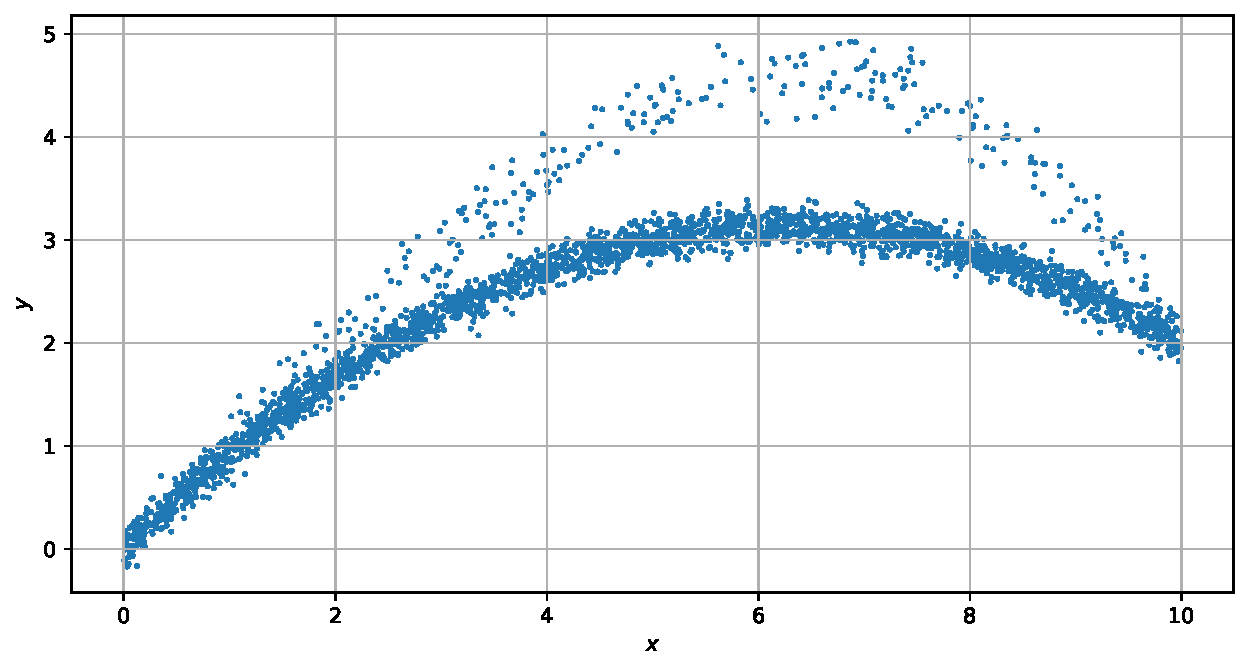
\includegraphics[width=\linewidth,height=0.6\paperheight,keepaspectratio=true]{data-only-f1.pdf}}
			\only<3>{ \centering 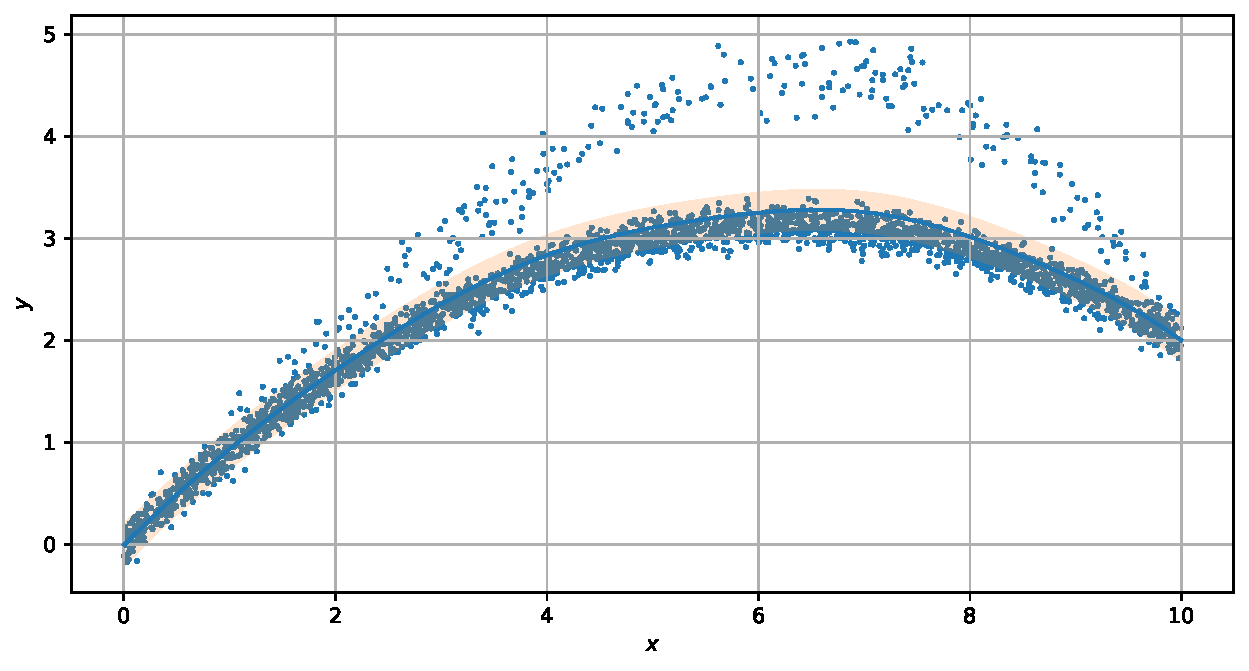
\includegraphics[width=\linewidth,height=0.6\paperheight,keepaspectratio=true]{fit-f1.pdf}}
			\only<4>{ \centering 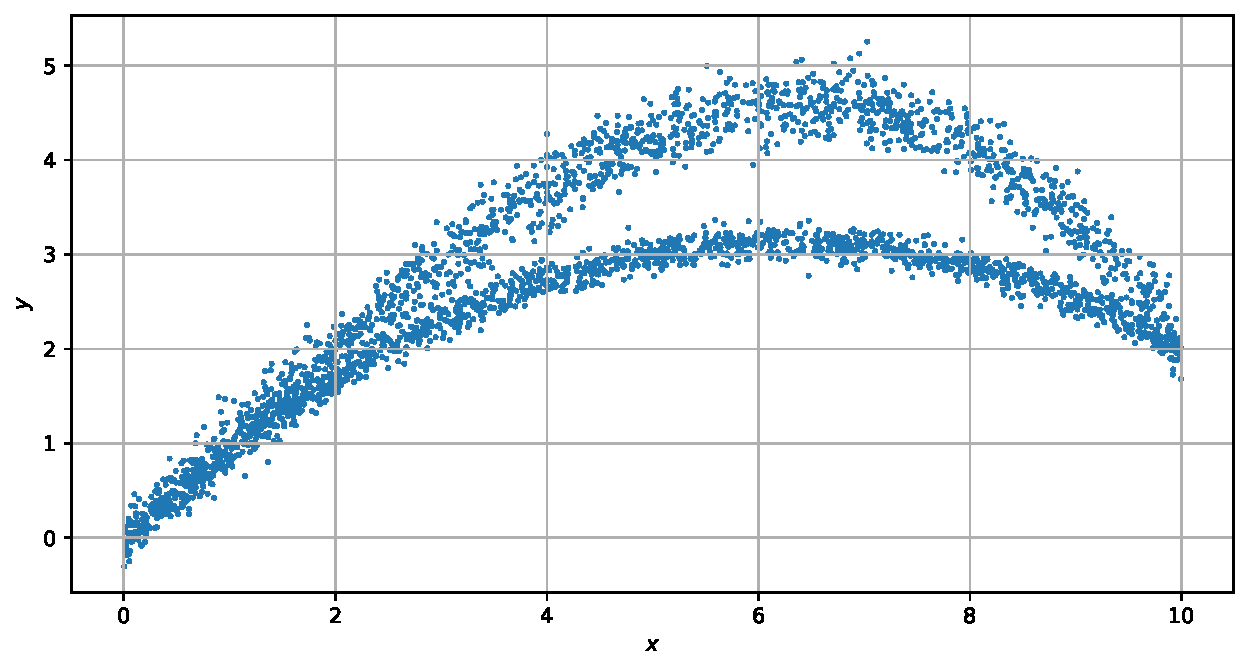
\includegraphics[width=\linewidth,height=0.6\paperheight,keepaspectratio=true]{data-only-f5.pdf}}
			\only<5>{ \centering 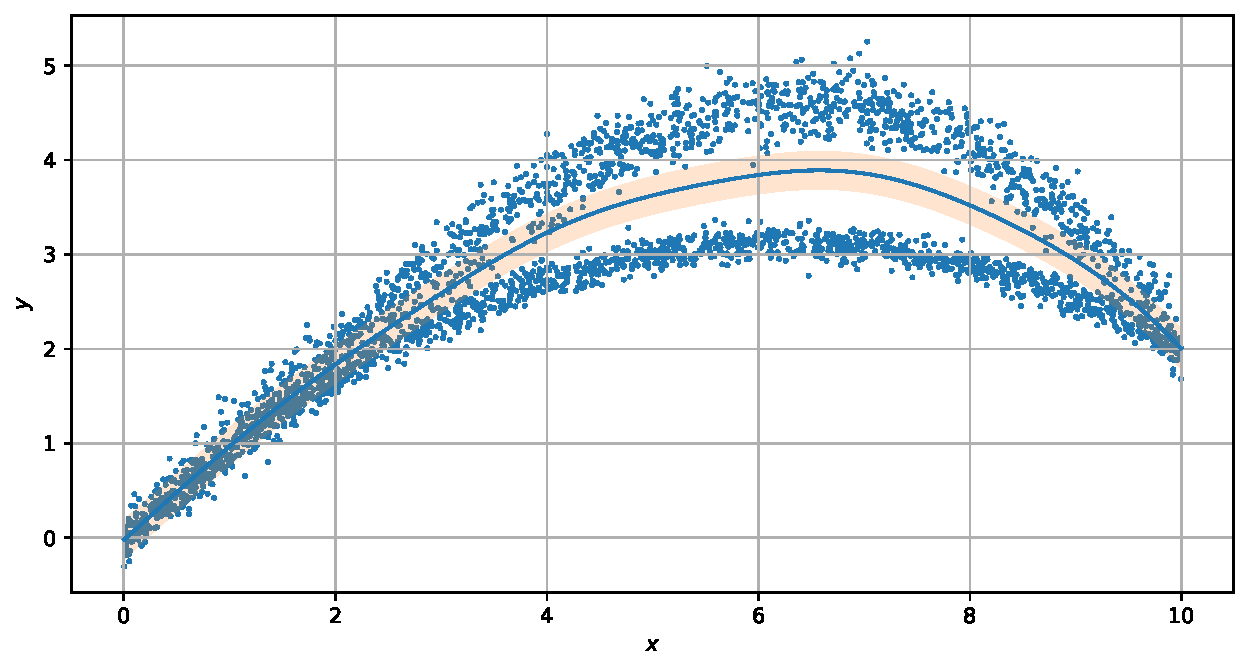
\includegraphics[width=\linewidth,height=0.6\paperheight,keepaspectratio=true]{fit-f5.pdf}}
		\end{frame}


		\begin{frame}{Machine Learning (Again)}
			There \textit{are} ML models which give distributions (Bayesian Neural Networks), but we may choose to avoid them:
			\begin{enumerate}
				\item Require lots of data (expensive - recall computing $\hat{M}$ is the bottleneck)
				\item Black boxes (aesthetically/scientifically dubious)
			\end{enumerate}
		\end{frame}
		\begin{frame}{Gaussian Processes}
			A modelling process where one assumes
			\begin{equation}
				\vec{y}(\vec{\pi}) \sim \mathcal{N}\left(\sum_i w_i(\pi) \vec{y}_i, \Sigma \right)
			\end{equation}
			% In short, compute an estimator of the mean, and then assume a Gaussian distribution at the end.

			Has many lovely properties, but fundamentally unsuitable for our work, as it assumes the distribution, rather than reconstructing it!


		\end{frame}

		\begin{frame}{Partition Models}
			Split the covariate space up into \textit{cells}

			\only<2>{ \centering 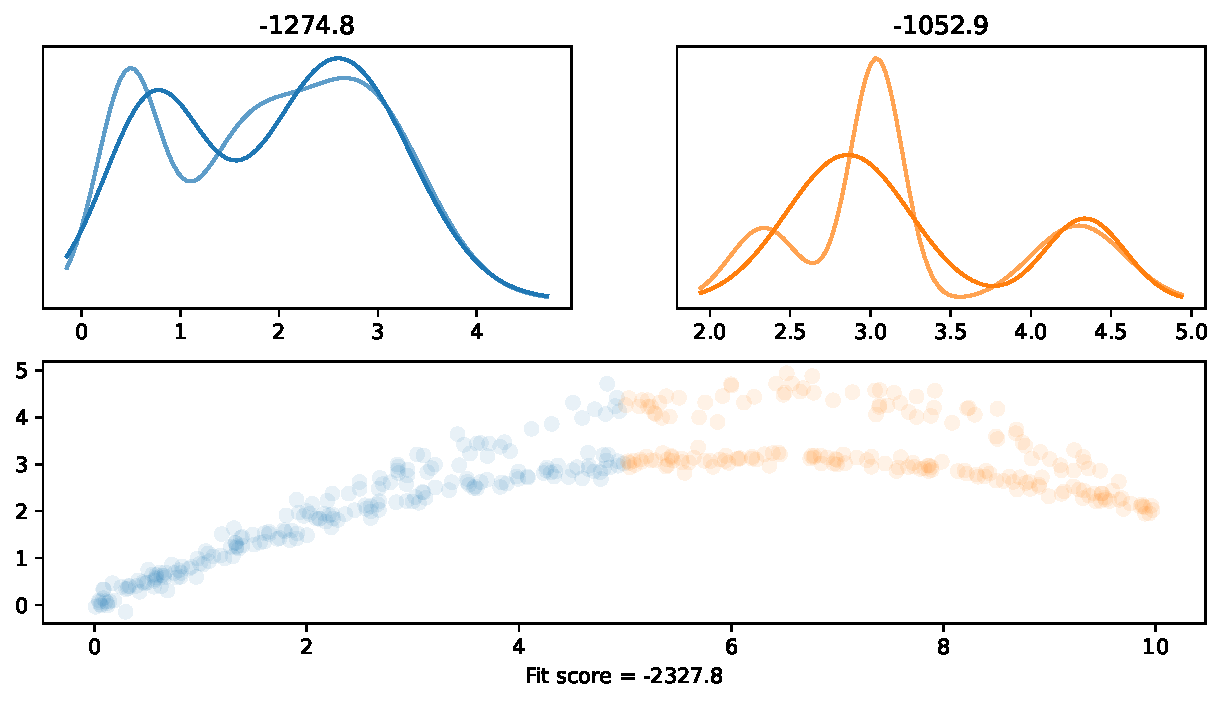
\includegraphics[width=\linewidth,height=0.6\paperheight,keepaspectratio=true]{partition-2-data.pdf}}
			\only<3>{ \centering 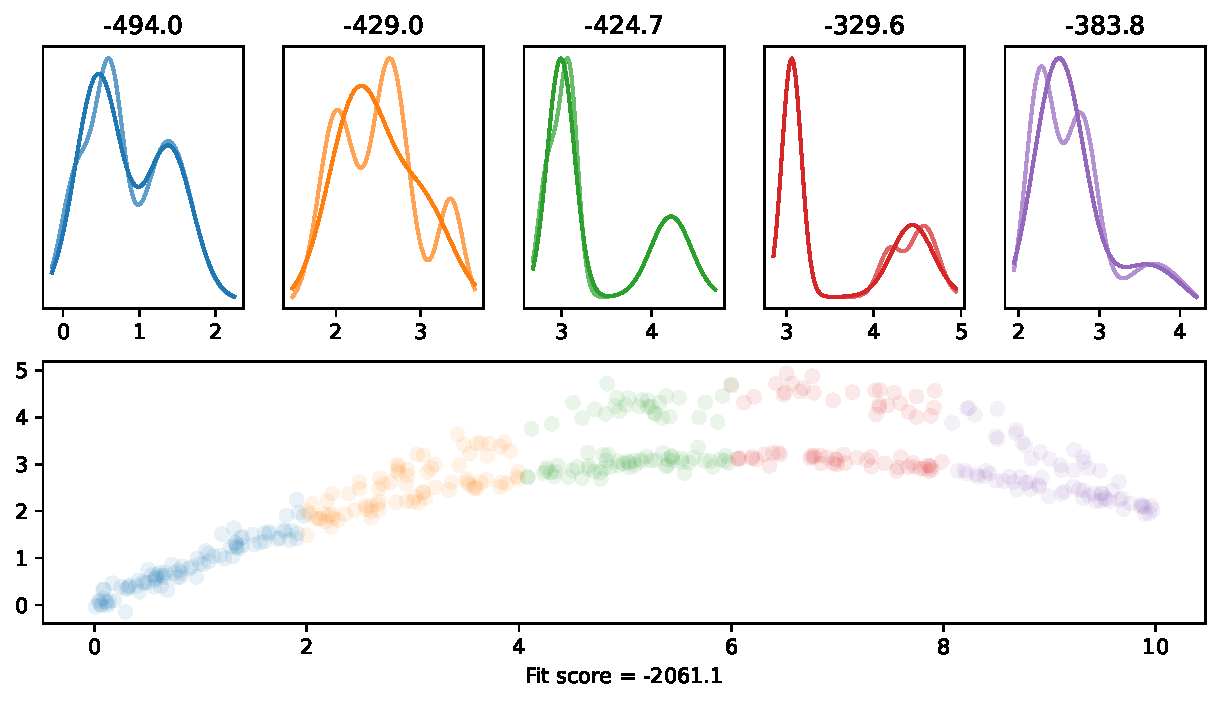
\includegraphics[width=\linewidth,height=0.6\paperheight,keepaspectratio=true]{partition-5-data.pdf}}
			\only<4>{ \centering 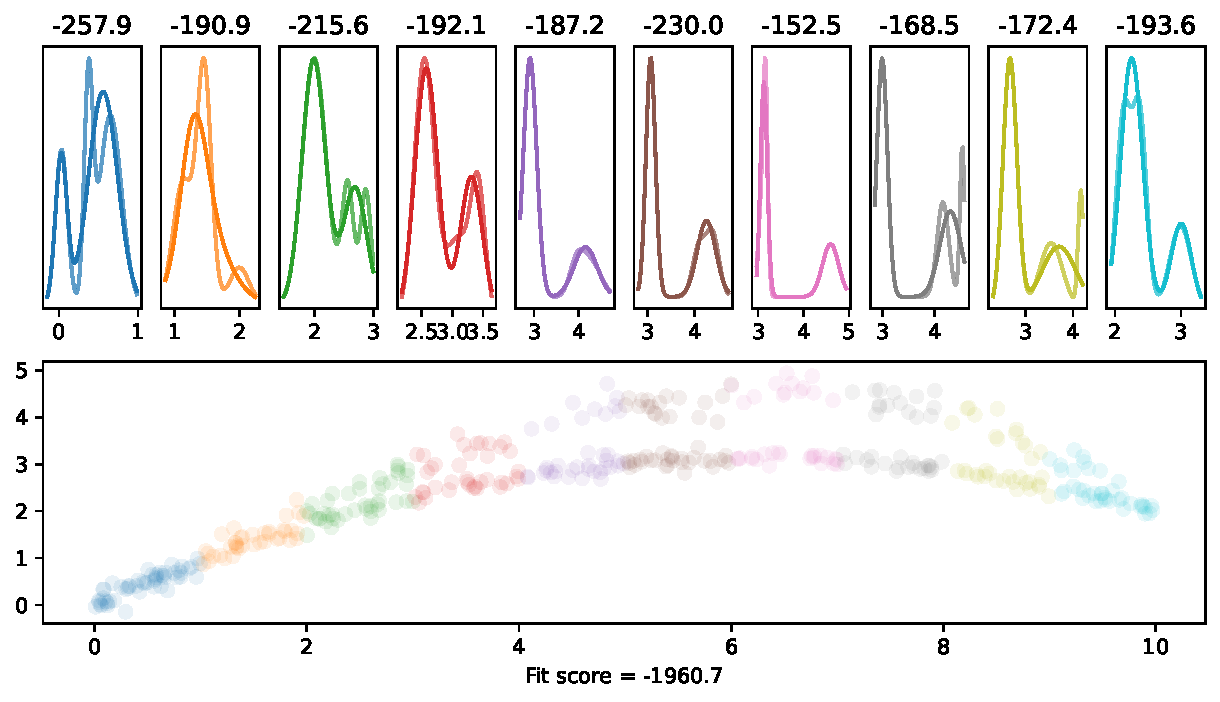
\includegraphics[width=\linewidth,height=0.6\paperheight,keepaspectratio=true]{partition-10-data.pdf}}
			\only<5>{ \centering 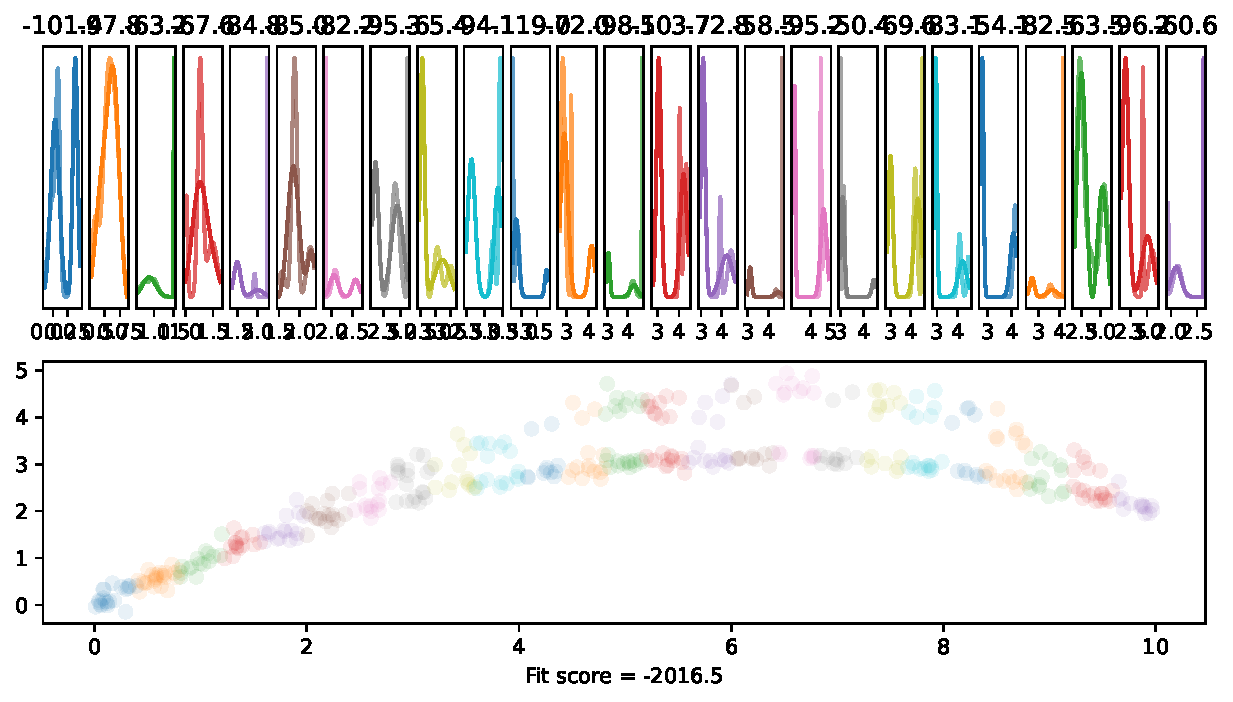
\includegraphics[width=\linewidth,height=0.6\paperheight,keepaspectratio=true]{partition-25-data.pdf}}
		\end{frame}
		\begin{frame}{Partition Models}
			In higher dimensions, the partioning gets harder!
			\begin{center}
				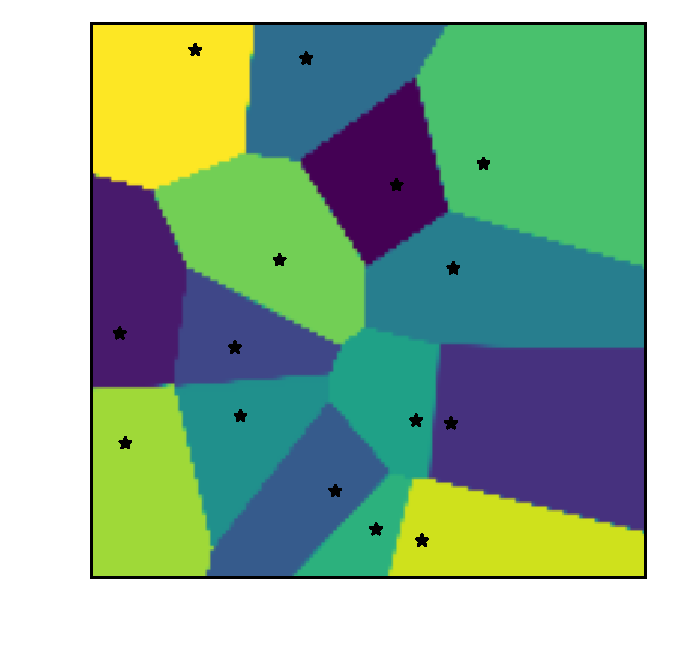
\includegraphics[scale=0.6]{tesselate}
			\end{center}
		\end{frame}

		\begin{frame}{Mixture of Experts}
			Instead of a hard partition, MoE probabilistically assign the `problem' to an `expert':
			\begin{equation}
				p(y | \vec{x}) = \sum_i w_i(\vec{x}) p_i
			\end{equation}
			The $w_i$ give different weights to the `expert opinion' at different points in covariate space, coming to a different consensus.

			Standard MoE uses Neural Networks to determine $w_i$ (via complex partitioning of a learned hyperplane projection)
		\end{frame}

		\begin{frame}{Models are not Emulators}
			\begin{block}{Important!}
				The above models \textit{are not emulators}. They provide ways to model the best-fit posterior distribution, conditioned on the observed data:

				$$ \text{Model}_{\vec{\Theta}}(\vec{x}) = p(\vec{y} | \vec{x}, \vec{\Theta})$$
			\end{block}
		\end{frame}
		\begin{frame}{Posterior Predictive Distribution}
			What we need it the \textit{posterior predictive} distribution. The distribution conditioned \textit{only} on the data:
			\pause\begin{equation}
				\text{Emulator}(\vec{x}) = p(\vec{y} | \vec{x}) = \int\text{Model}_{\vec{\Theta}}(\vec{x}) \mathrm d \vec{\Theta}
			\end{equation}
		\end{frame}

	\section{The FADE Emulator}
		\begin{frame}{Our Requirements}
			We needed an emulator which can:
			\begin{enumerate}
				\pitem Reconstruct probability distribution function
				\pitem Allow both smooth and near-discontinuous changes in behaviour
				\pitem Inherit `expert knowledge' to reduce training requirements
				\pitem Be interpretable and accessible
			\end{enumerate}
		\end{frame}

		\begin{frame}{Department of Experts}
			A middle ground between partitioning and MoE models. We allow each expert to belong to a `department' (a partition - which may have many experts within it), but also allow them to `spend time' between departments.

			The weight of an expert in the sum is then:
			\begin{equation}
				w_i(\vec{x}) = \sum_{\text{dep. } k} P(\vec{x} \in k) \times  \frac{P(i \in k) P(i \text{ knows } \vec{x})}{\sum_j P(j \in k) P(j \text{ knows } \vec{x})}
			\end{equation}
			These probabilities can be learned by the machine
		\end{frame}
		\begin{frame}{The Clever Bit}
			This reduces trivially down into a standard MoE, with model parameters $\vec{\Theta}$
			\begin{equation}
				p(\vec{x}|\vec{\Theta}) = \sum_w w_i(\vec{x} | \Theta) p_i(\vec{x} | \vec{\Theta})
			\end{equation}
			The clever bit is that we allow each department to have their own `grammar' that they use to talk to interpret the covariance space. The distance metric in each space is:
			\begin{equation}
				d_k(\vec{x}, \vec{y}) = \sqrt{(\vec{x} - \vec{y})\cdot G_k (\vec{x} - \vec{y})}
			\end{equation}
			Where $G_k$ is a learned distance metric unique to each cell.
		\end{frame}

		\begin{frame}{Why is this clever?}

			\begin{enumerate}
				\pitem Allows $w_i$ to encode highly nonlinear relationships in $\vec{x}$ \textit{without resorting to black-box machinery}.
				\pitem The metrics are easily interpreted as covariance measures localised within a department.
				\pitem Gives the same predictive power as a high dimensional hidden-layer neural network
				\pitem Constrained to produce `interpretable results'.
			\end{enumerate}
		\end{frame}

		\begin{frame}{A FADE Model}

			\begin{center}

				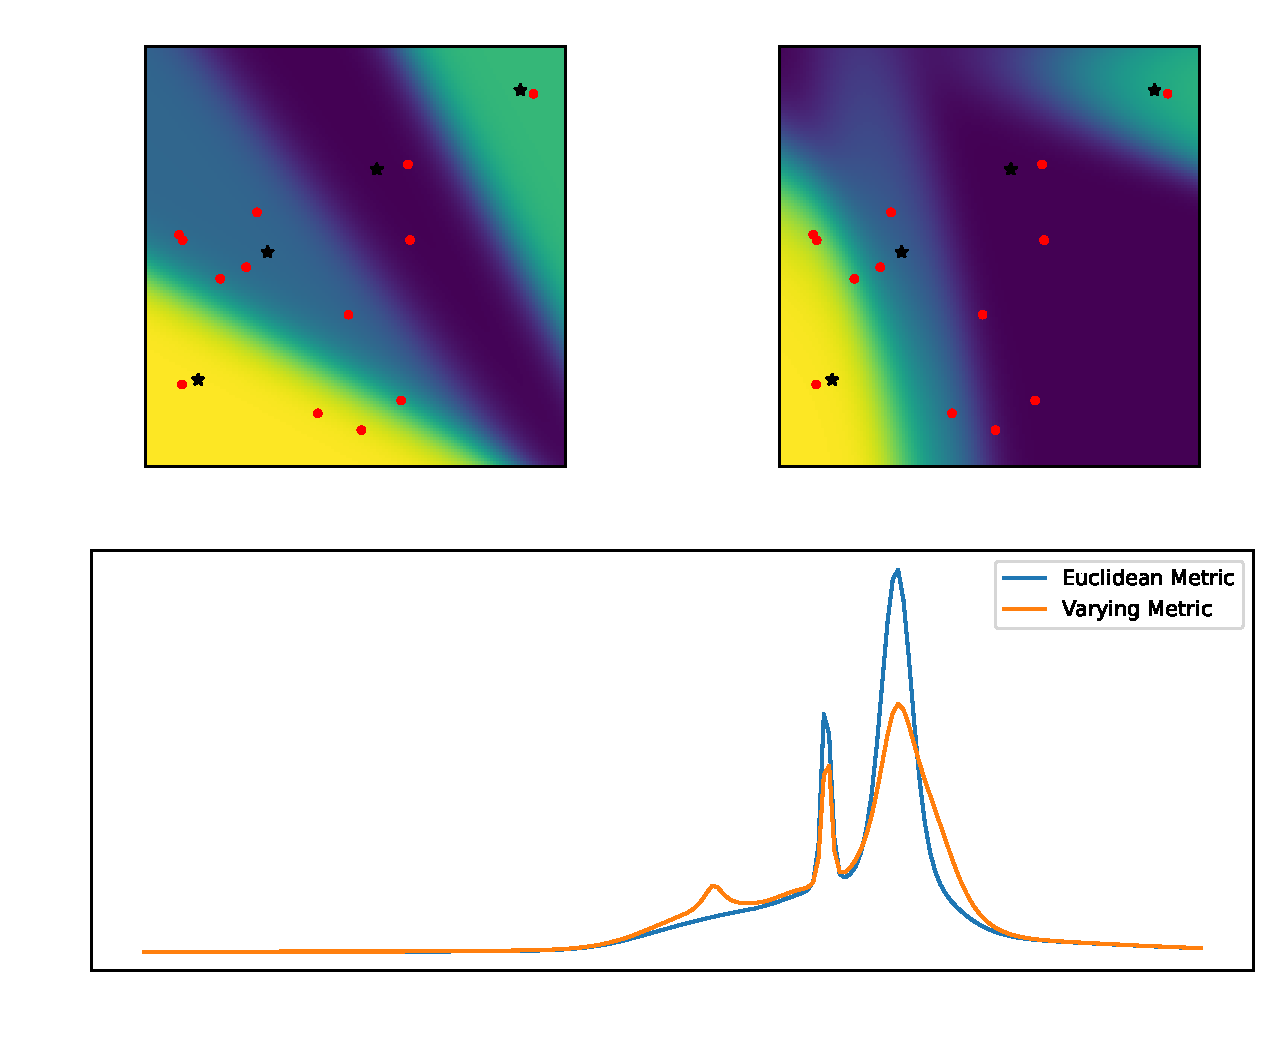
\includegraphics[scale=0.4]{metric_grids.pdf}
			\end{center}
		\end{frame}


	\section{The Projects}

		\begin{frame}{Project Ideas}
			As a group, we want to understand the capabilities (and limits) of our new tools: this is where you come in!

			\begin{description}
				\item[\scshape question one] What is the best way to train a FADE instance on a given dataset? Are there more or less optimal starting positions? Splits between training and validation data?
				\item[\scshape question two] What classes of models does FADE work best at emulating? What is it bad at? Can you show a transition point where FADE goes from good to bad, or vice versa?
				\item[\scshape question three] Can FADE be applied to other, real world models, in other fields? How accurate is it? Does the FADE setup bring advantages that a more naive emulation might miss?
			\end{description}
		\end{frame}

		\begin{frame}{Getting Started}
			\begin{block}{Important!} Don't try to get too advanced, too quickly: start small \& build your way up
			\end{block}
			\begin{enumerate}
				\item Familiarise yourself with the underlying theory of emulators: read the FADE paper
				\item Generate a synthetic dataset of a `model' that you have designed.
				\item Try and train a FADE instance to emulate your model: how good is it? What changes make it better or worse?
				\item Iterate and build on this, making the model more complex, and playing around with the FADE training and scoring.
			\end{enumerate}
		\end{frame}

		\begin{frame}{Tools \& Languages}
			This will be a computationally-heavy project, but there's no requirement to learn a language you aren't familiar with already.
			\begin{itemize}
				\item FADE itself is written in C++20.
				      \begin{enumerate}
					      \item You don't have to modify this code or alter it unless you want to explore this route.
					      \item You will, however, need to know how to set up config files for FADE, which will mean understanding what the options do.
				      \end{enumerate}
				\item When generating synthetic datasets, you may use whatever language you like (the output must be in a standardised format, for FADE to read it).
				\item When exploring other `real world' models, you'll need to ensure that you can actually run them
			\end{itemize}
		\end{frame}
\end{document}
